%
% This is the LaTeX template file for lecture notes for EE 382C/EE 361C.
%
% To familiarize yourself with this template, the body contains
% some examples of its use.  Look them over.  Then you can
% run LaTeX on this file.  After you have LaTeXed this file then
% you can look over the result either by printing it out with
% dvips or using xdvi.
%
% This template is based on the template for Prof. Sinclair's CS 270.

\documentclass[twoside]{article}
\usepackage{graphics}
\usepackage{float}
\usepackage{graphicx}
\usepackage{hyperref}
\setlength{\oddsidemargin}{0.25 in}
\setlength{\evensidemargin}{-0.25 in}
\setlength{\topmargin}{-0.6 in}
\setlength{\textwidth}{6.5 in}
\setlength{\textheight}{8.5 in}
\graphicspath{ {images/} }
\setlength{\headsep}{0.75 in}
\setlength{\parindent}{0 in}
\setlength{\parskip}{0.1 in}

%
% The following commands set up the lecnum (lecture number)
% counter and make various numbering schemes work relative
% to the lecture number.
%
\newcounter{lecnum}
\renewcommand{\thepage}{\thelecnum-\arabic{page}}
\renewcommand{\thesection}{\thelecnum.\arabic{section}}
\renewcommand{\theequation}{\thelecnum.\arabic{equation}}
\renewcommand{\thefigure}{\thelecnum.\arabic{figure}}
\renewcommand{\thetable}{\thelecnum.\arabic{table}}

%
% The following macro is used to generate the header.
%
\newcommand{\lecture}[4]{
   \pagestyle{myheadings}
   \thispagestyle{plain}
   \newpage
   \setcounter{lecnum}{#1}
   \setcounter{page}{1}
   \noindent
   \begin{center}
   \framebox{
      \vbox{\vspace{2mm}
    \hbox to 6.28in { {\bf EE 382C/361C: Multicore Computing
                        \hfill Fall 2016} }
       \vspace{4mm}
       \hbox to 6.28in { {\Large \hfill Lecture #1: #2  \hfill} }
       \vspace{2mm}
       \hbox to 6.28in { {\it Lecturer: #3 \hfill Scribe: #4} }
      \vspace{2mm}}
   }
   \end{center}
   \markboth{Lecture #1: #2}{Lecture #1: #2}
   %{\bf Disclaimer}: {\it These notes have not been subjected to the
   %usual scrutiny reserved for formal publications.  They may be distributed
   %outside this class only with the permission of the Instructor.}
   \vspace*{4mm}
}

%
% Convention for citations is authors' initials followed by the year.
% For example, to cite a paper by Leighton and Maggs you would type
% \cite{LM89}, and to cite a paper by Strassen you would type \cite{S69}.
% (To avoid bibliography problems, for now we redefine the \cite command.)
% Also commands that create a suitable format for the reference list.
\renewcommand{\cite}[1]{[#1]}
\def\beginrefs{\begin{list}%
        {[\arabic{equation}]}{\usecounter{equation}
         \setlength{\leftmargin}{2.0truecm}\setlength{\labelsep}{0.4truecm}%
         \setlength{\labelwidth}{1.6truecm}}}
\def\endrefs{\end{list}}
\def\bibentry#1{\item[\hbox{[#1]}]}

%Use this command for a figure; it puts a figure in wherever you want it.
%usage: \fig{NUMBER}{SPACE-IN-INCHES}{CAPTION}
\newcommand{\fig}[3]{
			\vspace{#2}
			\begin{center}
			Figure \thelecnum.#1:~#3
			\end{center}
	}
% Use these for theorems, lemmas, proofs, etc.
\newtheorem{theorem}{Theorem}[lecnum]
\newtheorem{lemma}[theorem]{Lemma}
\newtheorem{proposition}[theorem]{Proposition}
\newtheorem{claim}[theorem]{Claim}
\newtheorem{corollary}[theorem]{Corollary}
\newtheorem{definition}[theorem]{Definition}
\newenvironment{proof}{{\bf Proof:}}{\hfill\rule{2mm}{2mm}}

% **** IF YOU WANT TO DEFINE ADDITIONAL MACROS FOR YOURSELF, PUT THEM HERE:

\begin{document}
%FILL IN THE RIGHT INFO.
%\lecture{**LECTURE-NUMBER**}{**DATE**}{**LECTURER**}{**SCRIBE**}
\lecture{22}{November 10}{Vijay Garg}{Zihan Yang}
%\footnotetext{These notes are partially based on those of Nigel Mansell.}

% **** YOUR NOTES GO HERE:

% Some general latex examples and examples making use of the
% macros follow.  
%**** IN GENERAL, BE BRIEF. LONG SCRIBE NOTES, NO MATTER HOW WELL WRITTEN,
%**** ARE NEVER READ BY ANYBODY.

\section*{Agenda}
This lecture is a general introduction of Stream, a new abstract layer in Java 8:
\begin{itemize}
    \item Stream basics
    \item Stream and Collection
    \item Simple examples of Stream
    \item 2 puzzles
\end{itemize} 

\section{Introduction}
A stream is a sequence of elements supporting sequential and parallel aggregate operations. 

To perform a computation, stream operations are composed into a stream pipeline. A stream pipeline consists of a source (which might be an array, a collection, a generator function, an I/O channel, etc), zero or more intermediate operations (which transform a stream into another stream, such as filter(Predicate)), and a terminal operation (which produces a result or side-effect, such as count() or forEach(Consumer)). 
\begin{figure}[h]
\centering
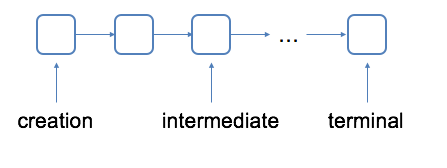
\includegraphics[scale=0.8]{pipeline}
\caption{Stream in pipeline fashion}
\label{fig:1}
\end{figure}

Stream pipelines may execute either sequentially or in parallel. This execution mode is a property of the stream. Streams are created with an initial choice of sequential or parallel execution. For example, Collection.stream() creates a sequential stream, and Collection.parallelStream() creates a parallel one. Operations on a sequential stream are processed in serial by one thread. Operations on parallel stream stream are processed in parallel by multiple threads.
Most of the methods in the Streams API produce sequential streams by default. 

\section{Stream basics}

\begin{center}
\begin{tabular}{ |c|c| } 
 \hline
 Stream & Collection  \\
 \hline
 Concept of time & Concept of space  \\ 
 Use it only once & Use it any time  \\ 
 Focus on aggregate operations & Focus on how to store and access elements \\ 
 Number of elements could be infinite & Always finite  \\ 
 Lazy evaluation & All the elements are always there  \\ 
 \hline
\end{tabular}
\end{center}

In order to compare stream with collection, Fig 22.2 shows a snippet of code in which we square every odd element in an array and return its sum using collection and stream. With the help of stream, we can implement it just in one line. By contrast, the collection implementation is much longer.
 
\begin{figure}[h]
\centering
\includegraphics[scale=0.8]{Fig1}
\caption{Comparison between Collection and Stream }
\label{fig:1}
\end{figure}

Even though Streams and Collections seem to share some superficial similarities. They actually serve for different goals. Collections are primarily concerned with the efficient management of, and access to, their elements. By contrast, streams do not provide a means to directly access or manipulate their elements and are instead concerned with declaratively describing their source and the computational operations which will be performed in aggregate on that source. 

Besides, streams are not reusable. A stream can't be reused after calling a terminal operation. Look at the code in Fig 22.3,  everything works well in line 13, but the line 16 should be commented because the streams can only be consumed once. However, all the elements in collections are always there and could be operated at any time. Streams are lazy because computation on the source data is only performed when the terminal operation is initiated, and source elements are consumed only as needed. To some extend, stream is more like a concept of time while collection is of concept of space. 

\begin{figure}[h]
\centering
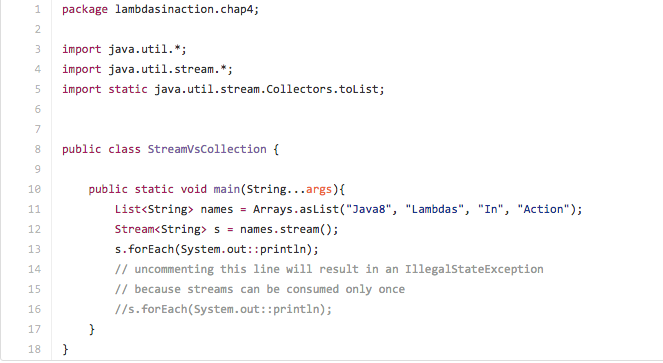
\includegraphics[scale=0.6]{streamVScollection}
\caption{A stream is not resuable }
\label{fig:2}
\end{figure}

Another difference is that a collection cannot represent a group of infinite elements whereas a stream can. A stream can pull its elements from a data source. The source can be a collection, an I/0 channel or a function which can generate infinite number of elements.


\section{Simple examples of Stream}
\subsection{Java Stream Create}
We can create stream in the following ways:
\begin{itemize}
    \item Create Streams from values
    \item Create Streams from Empty streams
    \item Create Streams from functions
    \item Create Streams from arrays
    \item Create Streams from collections
    \item Create Streams from files
    \item Create Streams from other sources
\end{itemize} 
For detailed descriptions and examples,  please refer to: \url{http://www.java2s.com/Tutorials/Java/Java_Stream/0040__Java_Stream_Create.htm}

\subsection{Java Stream opearations}
There are two types of operations:terminal and intermediate. The commonly used stream operations are listed as follows:
\begin{itemize}
\item Distinct(intermediate):
Returns a stream consisting of the distinct elements by checking equals() method.
\item Filter(intermediate):
Returns a stream that match the specified predicate.
\item FlatMap(intermediate):
Produces a stream flattened.
\item Limit(intermediate):
truncates a stream by number.
\item Map(intermediate):
Performs one-to-one mapping on the stream
\item Peek(intermediate):
Applies the action for debugging.
\item Skip(intermediate):
Discards the first n elements and returns the remaining stream. If this stream contains fewer than requested, an empty stream is returned.
\item Sorted(intermediate):
Sort a stream according to natural order or the specified Comparator. For an ordered stream, the sort is stable.
\item allMatch(terminal):
Returns true if all elements in the stream match the specified predicate, false otherwise. Returns true if the stream is empty.
\item anyMatch(terminal):
Returns true if any element in the stream matches the specified predicate, false otherwise. Returns false if the stream is empty.
\item findAny(terminal):
Returns any element from the stream. Returns an empty Optional object for an empty stream.
\item findFirst(terminal):
Returns the first element of the stream. For an ordered stream, it returns the first element; for an unordered stream, it returns any element.
\item noneMatch(terminal):
Returns true if no elements in the stream match the specified predicate, false otherwise. Returns true if the stream is empty.
\item forEach(terminal):
Applies an action for each element in the stream.
\item reduce(terminal):
Applies a reduction operation to computes a single value from the stream.
\end{itemize} 

For detailed descriptions and examples,  please refer to: \url{http://www.java2s.com/Tutorials/Java/Java_Stream/0200__Java_Stream_Operations.htm}

In the class, Prof.Garg walked us through some of the operations and concepts of streams using the examples on the github: \url{https://github.com/java8/Java8InAction}, including:\\
\begin{itemize}
\item syntax of \textbf{lambda function}(\url{https://github.com/java8/Java8InAction/blob/master/src/main/java/lambdasinaction/chap3/Lambdas.java})
\item \textbf{filter} operation(\url{https://github.com/java8/Java8InAction/blob/master/src/main/java/lambdasinaction/chap1/FilteringApples.java})
\item \textbf{sort} operation(\url{https://github.com/java8/Java8InAction/blob/master/src/main/java/lambdasinaction/chap3/Sorting.java})
\item \textbf{reduce} operation(\url{https://github.com/java8/Java8InAction/blob/master/src/main/java/lambdasinaction/chap5/Reducing.java}) 
\item mechanism of \textbf{lazy evaluation} of stream(\url{https://github.com/java8/Java8InAction/blob/master/src/main/java/lambdasinaction/chap5/Laziness.java})
\item \textbf{parallel streams}(\url{https://github.com/java8/Java8InAction/blob/master/src/main/java/lambdasinaction/chap7/ParallelStreams.java})
\end{itemize} 

 



\section*{References}
\beginrefs
\bibentry{1}{\sc Tutorials on Java Streaming},
\url{http://www.java2s.com/Tutorials/Java/Java_Stream/index.htm}
\bibentry{2}{\sc Java8InAction on github},
\url{https://github.com/java8/Java8InAction/tree/master/src}
\bibentry{3}{\sc Documentation of Java stream on Oracle Help Center},
\url{https://docs.oracle.com/javase/8/docs/api/java/util/stream/Stream.html}
\endrefs


\end{document}





